\documentclass{standalone}

\usepackage{tikz}
\usetikzlibrary{matrix,chains,positioning,decorations.pathreplacing,arrows}

\begin{document}
\pagestyle{empty}

\def\layersep{2.5cm}

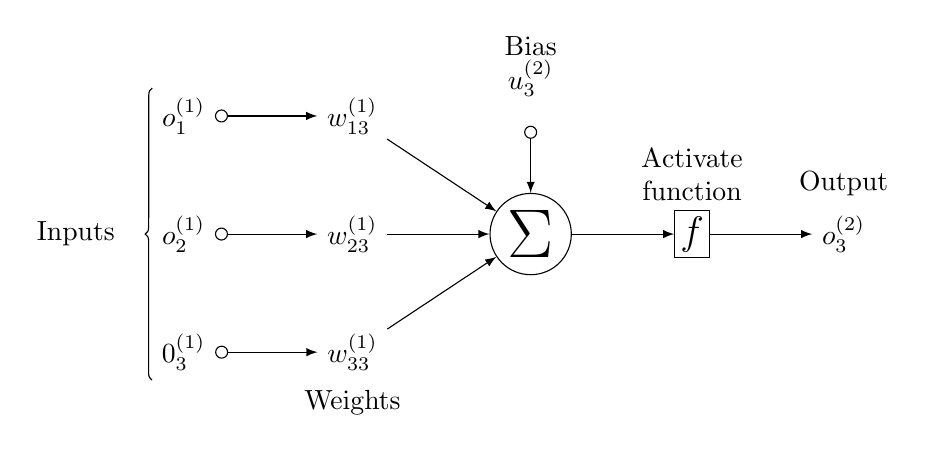
\begin{tikzpicture}[
init/.style={
  draw,
  circle,
  inner sep=2pt,
  font=\Huge,
  join = by -latex
},
squa/.style={
  draw,
  inner sep=2pt,
  font=\Large,
  join = by -latex
},
start chain=2,node distance=13mm
]
\node[on chain=2]
  (x2) {$o^{(1)}_2$};
\node[on chain=2,join=by o-latex]
  {$w^{(1)}_{23}$};
\node[on chain=2,init] (sigma)
  {$\displaystyle\Sigma$};
\node[on chain=2,squa,label=above:{\parbox{2cm}{\centering Activate \\ function}}]
  {$f$};
\node[on chain=2,label=above:Output,join=by -latex]
  {$o^{(2)}_3$};
\begin{scope}[start chain=1]
\node[on chain=1] at (0,1.5cm)
  (x1) {$o^{(1)}_1$};
\node[on chain=1,join=by o-latex]
  (w1) {$w^{(1)}_{13}$};
\end{scope}
\begin{scope}[start chain=3]
\node[on chain=3] at (0,-1.5cm)
  (x3) {$0^{(1)}_3$};
\node[on chain=3,label=below:Weights,join=by o-latex]
  (w3) {$w^{(1)}_{33}$};
\end{scope}
\node[label=above:\parbox{2cm}{\centering Bias \\ $u^{(2)}_3$}] at (sigma|-w1) (b) {};

\draw[-latex] (w1) -- (sigma);
\draw[-latex] (w3) -- (sigma);
\draw[o-latex] (b) -- (sigma);

\draw[decorate,decoration={brace,mirror}] (x1.north west) -- node[left=10pt] {Inputs} (x3.south west);
\end{tikzpicture}
% End of code
\end{document}
